\section{§ 9. Autoencoder}

\subsection{Unsupervised Learning}

\begin{frame}[allowframebreaks]

\begin{mydefinitionblock}{9.1}{Unsupervised Learning}
    \textbf{Unsupervised learning} utilizes data $X_{1}, \ldots, X_{N}$ to learn the "structure" of the data. No labels are utilized.

    There are a wide range of unsupervised learning tasks. In this class, we discuss just a few.

    Generally, unsupervised learning tasks tend to have more mathematical complexity.
\end{mydefinitionblock}

\end{frame}

\begin{frame}[allowframebreaks]

\begin{myconceptblock}{9.2}{Many data has low-dimensional latent representation, and the task is to find it.}
    Many high-dimensional data has some underlying low-dimensional structure.
    (One can model this assumption as data residing in a low dimensional manifold and utilize ideas from differential geometry. We won’t pursue this direction)

    If you randomly generate the pixels of a color image $X \in \mathbb{R}^{3 \times m \times n}$, it will likely make no sense. Only a very small subset of pixel values correspond to meaningful images.

    In machine learning, especially in unsupervised learning, finding a "meaningful" low dimensional latent representation is of interest.

    A good lower-dimensional representation of the data implies you have a good understanding of the data.
\end{myconceptblock}

\end{frame}

\subsection{Definition of Autoencoder}

\begin{frame}[allowframebreaks]

\begin{mydefinitionblock}{9.3}{Autoencoder}
    An \textbf{autoencoder (AE)} has encoder $E_{\theta}: \mathbb{R}^{n} \rightarrow \mathbb{R}^{r}$ and decoder $D_{\varphi}: \mathbb{R}^{r} \rightarrow \mathbb{R}^{n}$ networks, where $r \ll n$. (If $r \geq n$, AE learns identity mapping, so pointless.) The two networks are trained through the loss

    $$
    \mathcal{L}(\theta, \varphi)=\sum_{i=1}^{N}\left\|X_{i}-D_{\varphi}\left(E_{\theta}\left(X_{i}\right)\right)\right\|^{2}
    $$

    The low-dimensional output $E_{\theta}(X)$ is the latent vector. The encoder performs dimensionality reduction.

    The autoencoder can be thought of as a deep non-linear generalization of the principle component analysis (PCA).

    \begin{figure}[H]
        \centering
        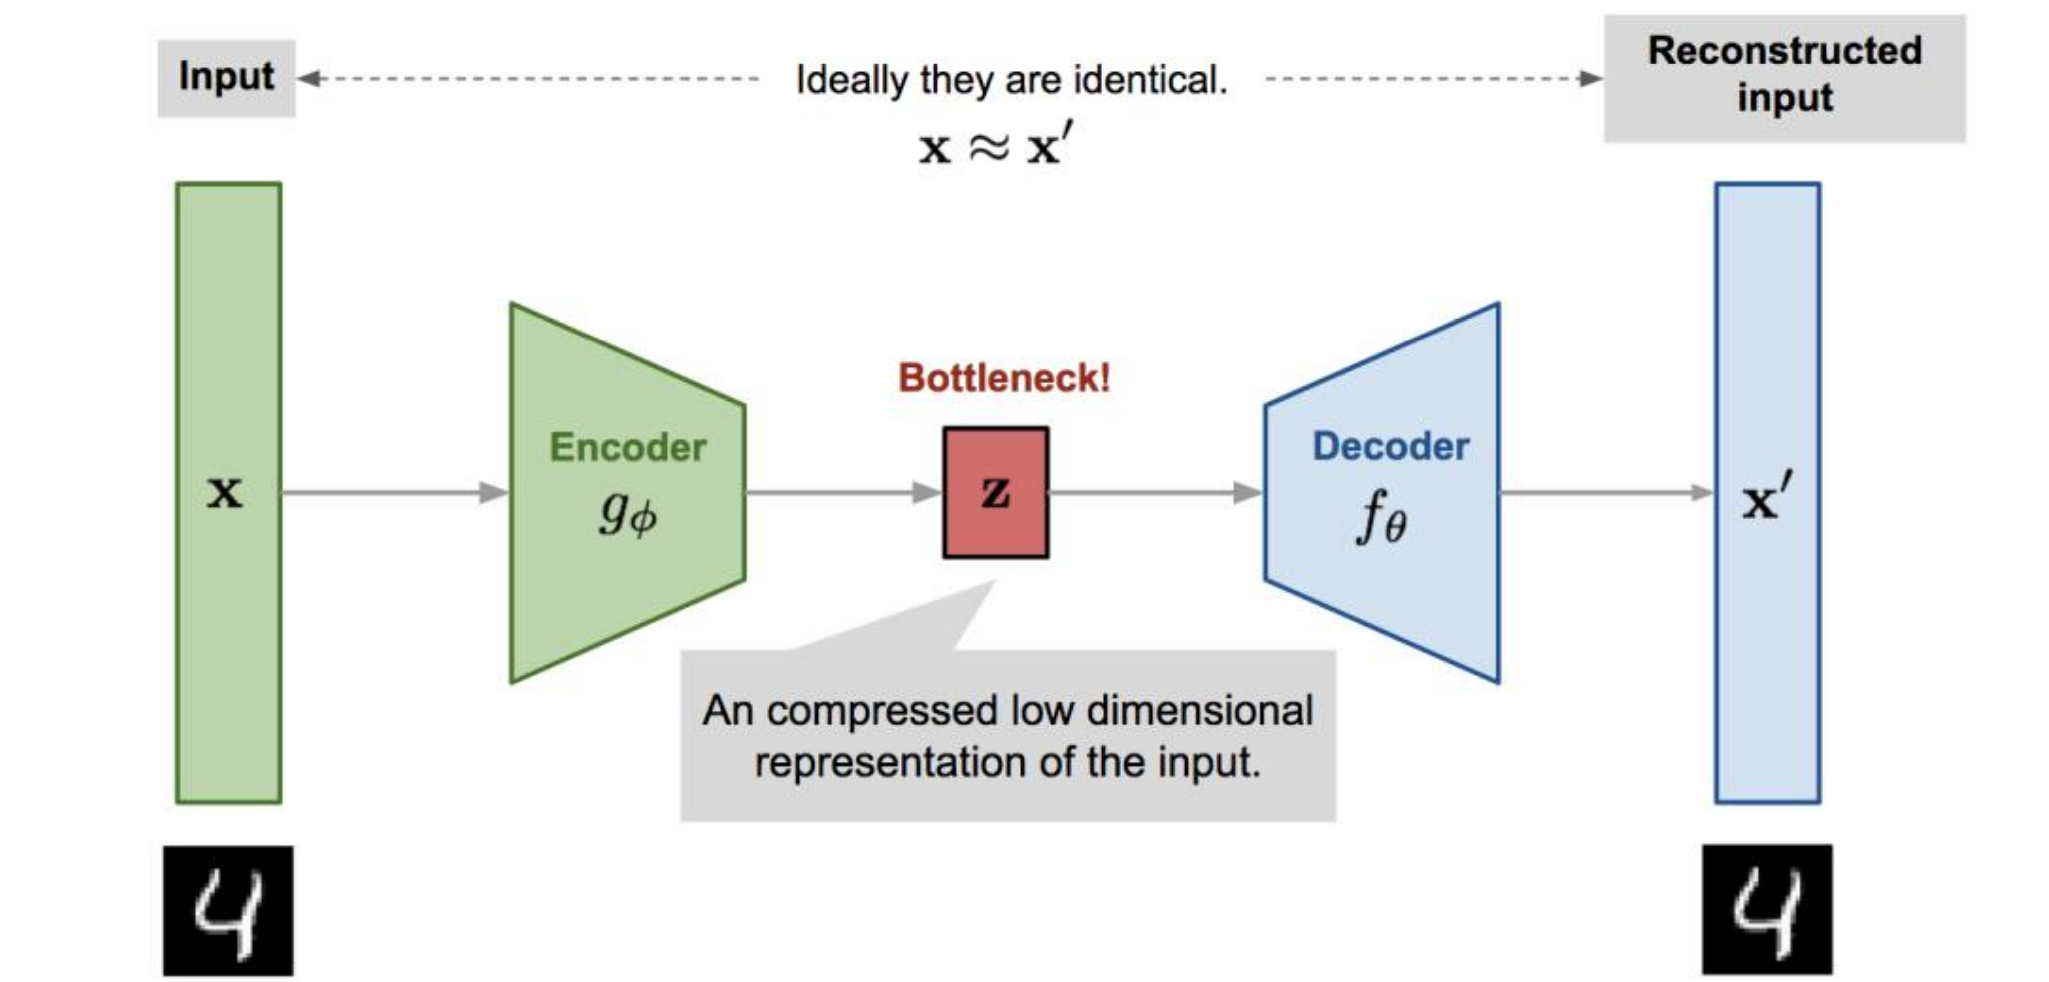
\includegraphics[width=0.8\textwidth]{.././assets/9.1.png}
    \end{figure}

    (G. E. Hinton and R. R. Salakhutdinov, Reducing the dimensionality of data with neural networks, Science, 2006.)
\end{mydefinitionblock}

\end{frame}

\subsection{Applications of Autoencoder}

\begin{frame}[allowframebreaks]

\begin{myconceptblock}{9.4}{Applications of AE}
    Autoencoders can be used to denoise or reconstruct corrupted images.

    \begin{figure}[H]
        \centering
        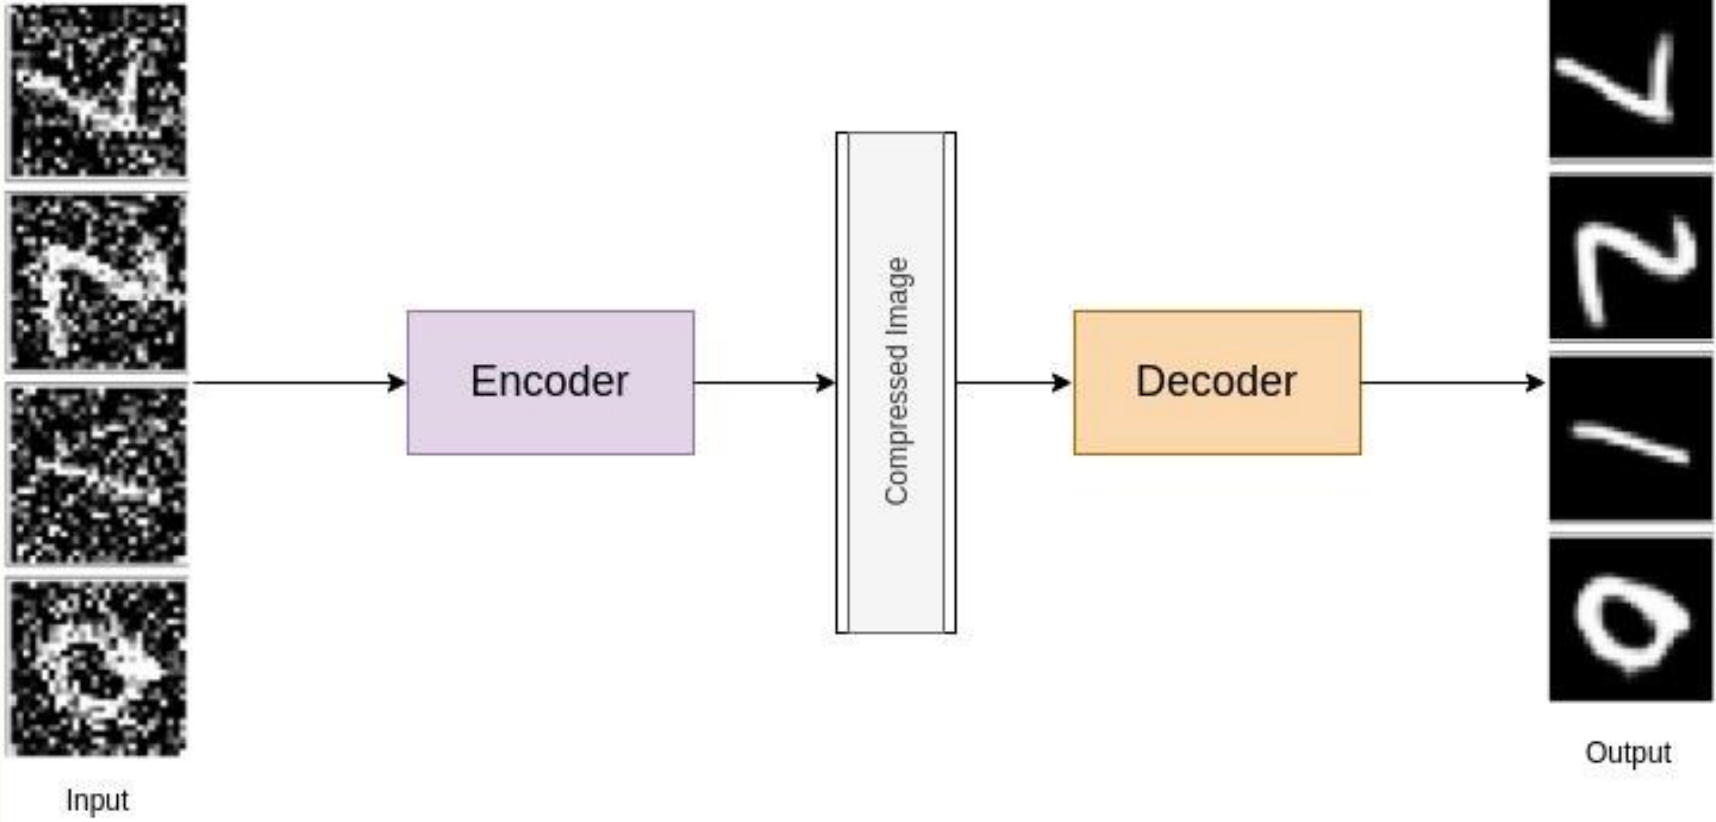
\includegraphics[width=0.7\textwidth]{.././assets/9.2.png}
    \end{figure}

    \begin{figure}[H]
        \centering
        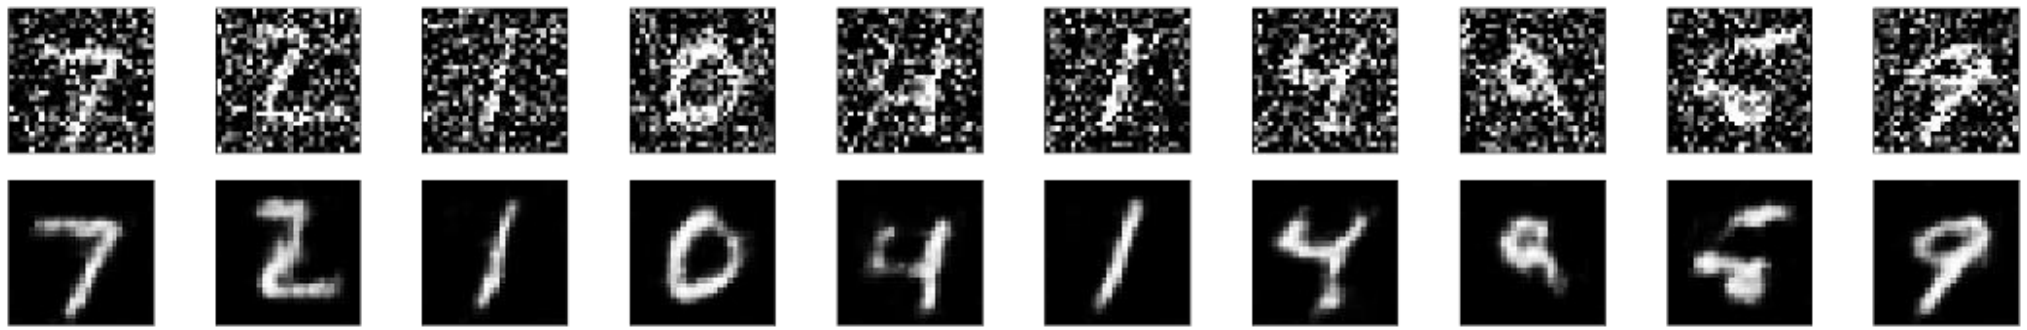
\includegraphics[width=1.0\textwidth]{.././assets/9.3.png}
    \end{figure}

    (P. Vincent, H. Larochelle, I. Lajoie, Y. Bengio, and P.-A. Manzagol, Stacked denoising autoencoders: Learning useful representations in a deep network with a local denoising criterion, JMLR, 2010.
    G. Nishad, Reconstruct corrupted data using Denoising Autoencoder, Medium, 2020.)
\end{myconceptblock}

\end{frame}

\begin{frame}[allowframebreaks]

\begin{myconceptblock}{9.5}{Applications of AE}
    Once an AE has been trained, storing the latent variable representation, rather than the original image can be used as a compression mechanism.

    More generally, latent variable representations can be used for video compression.
    (\href{https://youtu.be/NqmMnjJ6GEg}{link})
\end{myconceptblock}

\end{frame}

\begin{frame}[allowframebreaks]

\begin{myconceptblock}{9.6}{Applications of AE}
    Train an AE and then perform clustering on the latent variables. For the clustering algorithm, one can use things like k-means, which groups together.

    Clustering is also referred to as unsupervised classification. Without labels, we want the group "similar" data.

    \begin{figure}[H]
        \centering
        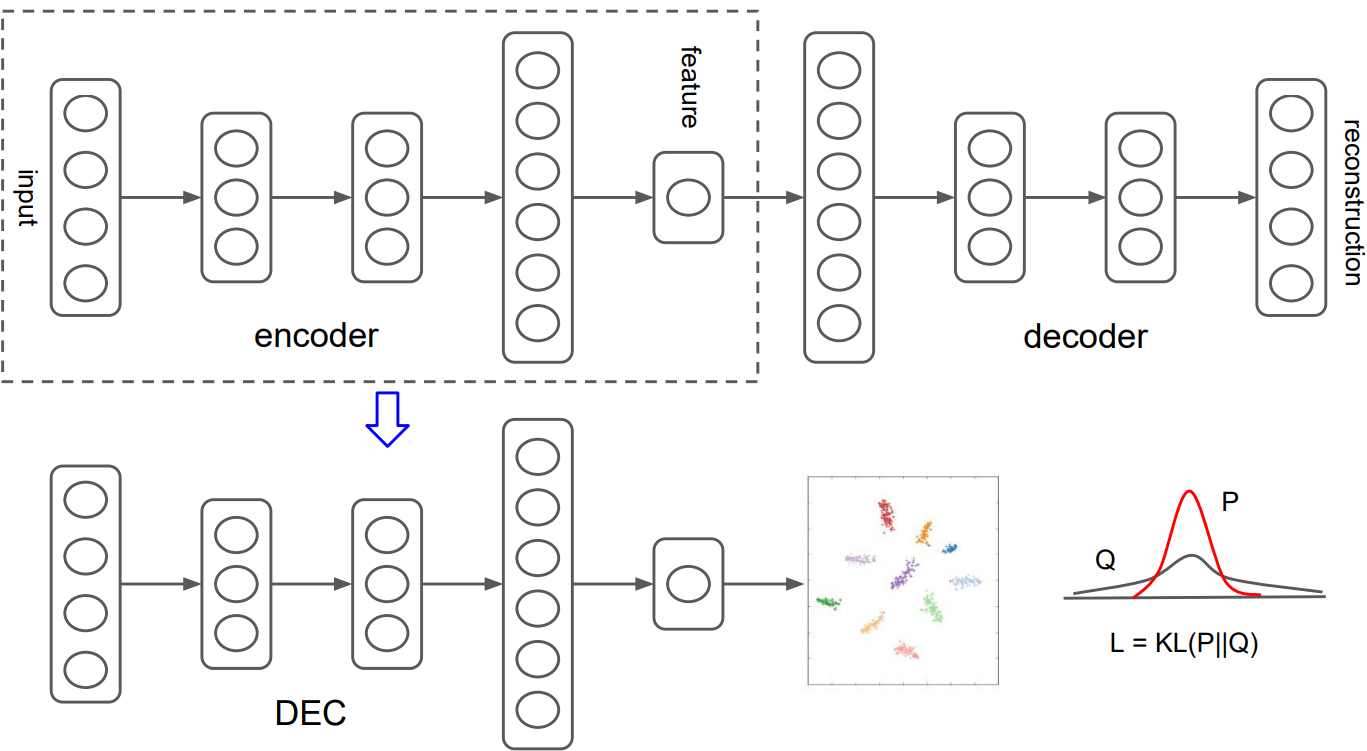
\includegraphics[width=0.7\textwidth]{.././assets/9.4.png}
    \end{figure}

    \begin{figure}[H]
        \centering
        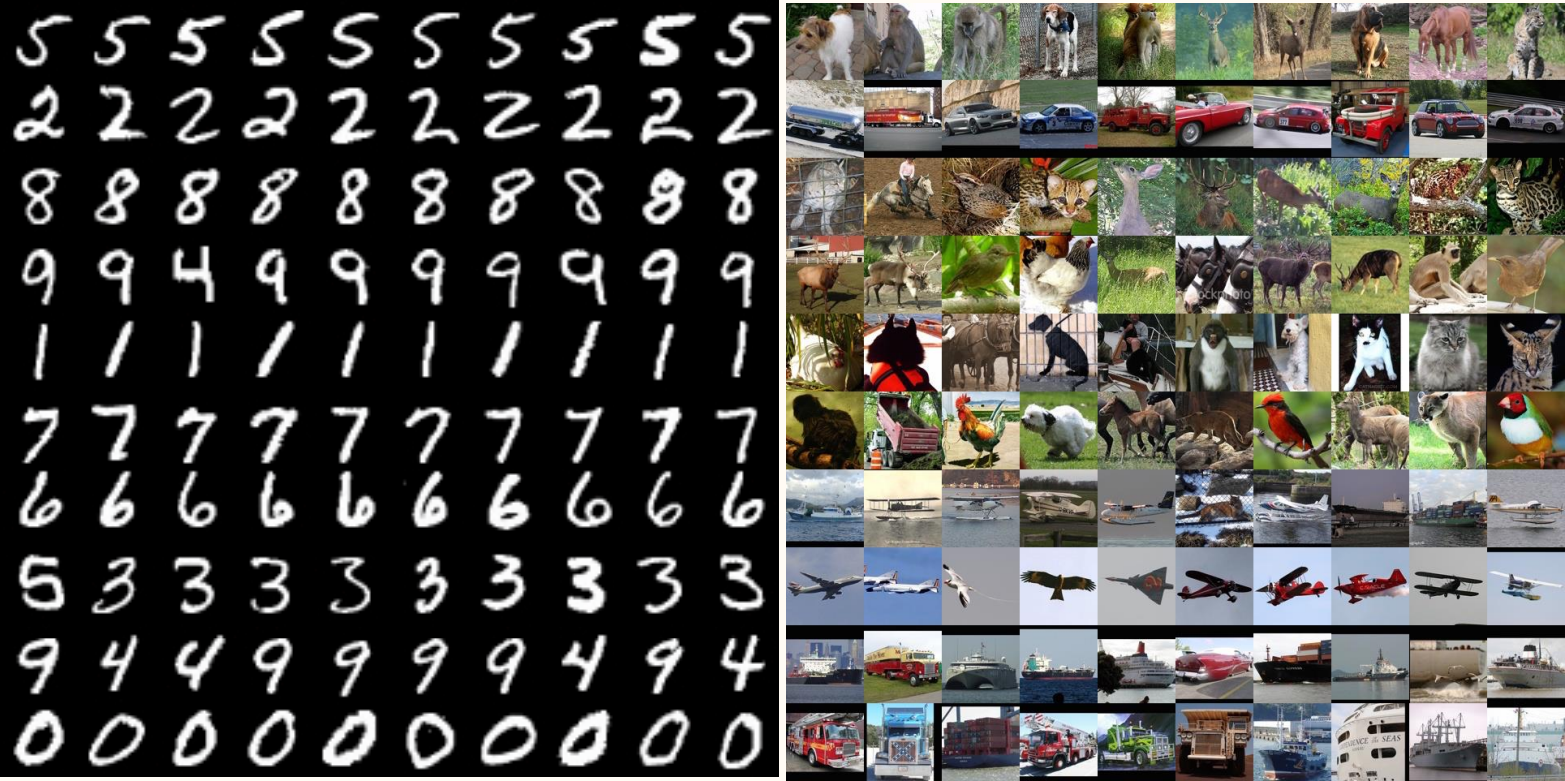
\includegraphics[width=1.0\textwidth]{.././assets/9.5.png}
    \end{figure}

    (J. Xie, R. Girshick, and A. Farhadi, Unsupervised deep embedding for clustering analysis, ICML, 2016.)
\end{myconceptblock}

\end{frame}

\begin{frame}[allowframebreaks]

\begin{myconceptblock}{9.7}{Anomaly/Outlier Detection}
    \textbf{Problem}: detecting data that is significantly different from the data seen during training.

    \textbf{Insight}: AE should not be able to faithfully reconstruct novel data.

    \textbf{Solution}: Train an AE and define the score function to be the reconstruction loss:

    $$
    s(X)=\left\|X-D_{\varphi}\left(E_{\theta}(X)\right)\right\|^{2}
    $$

    If score is high, determine the datapoint to be an outliner.

    (S. Hawkins, H. He, G. Williams, and R. Baxter, Outlier detection using replicator neural networks, DaWaK, 2002.)
\end{myconceptblock}

\end{frame}
